\section{Corazones}

\begin{figure}[htbp]
\begin{center}
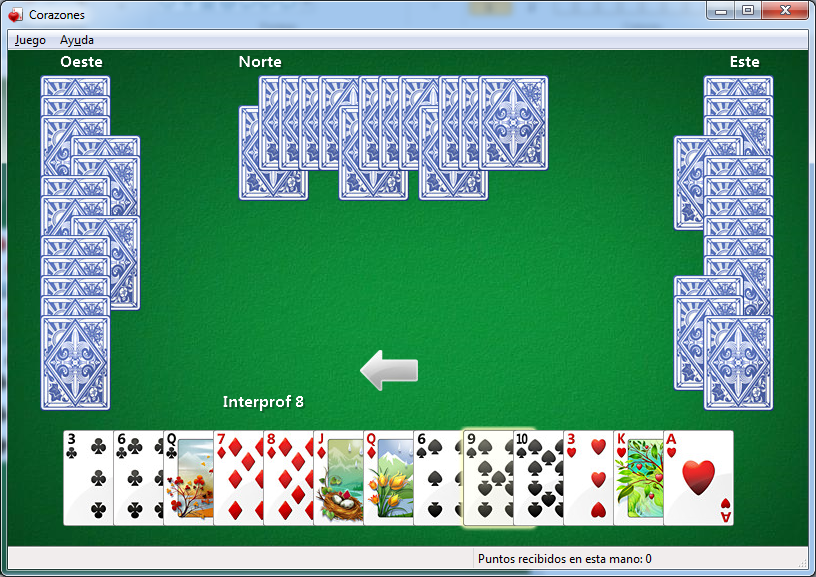
\includegraphics[width=.60\textwidth]{./imagenes/Corazones.png}
\caption{Corazones}
\label{Corazones}
\end{center}
\end{figure}
Corazones\footnote{\url{http://www.magnojuegos.com/juegosonline/corazones/}} es un juego de cartas cuyo objetivo es acabar la partida con el mínimo de puntos posibles. Es una evolución del original "Dama de Picas" francés. El juego estándar se realiza con una baraja francesa y cuatro jugadores. Se ha popularizado mucho a partir de su inclusión en el sistema operativo Windows.
En la figura \ref{Corazones} puede ver una implementación del juego.
La premisa del juego es simple: Tener la menor cantidad de puntos al final de las partidas.

\subsubsection{¿Por qué es uno de mis juegos favoritos?}
\begin{itemize}
\item[Veronica Pozo] Porque es uno de los primeros juegos que venían instalados en Windows y crecí jugando este juego. Es un juego sencillo y facil de entender para cualquier edad. Era muy útil cuando te aburrías de Buscaminas y Carta Blanca. Crecer sin internet nos llevó a aprovechar los juegos que teníamos a la mano. Los juegos de cartas como Solitario, Carta Blanca y Corazones fueron parte de nuestra infancia y a pesar de los nuevos juegos como Solitario Spider creo que los clásicos, con los que crecimos, siempre tendrán unos minutitos de nuestro tiempo.
\end{itemize}
